% !TeX program = xelatex
% !TeX encoding = UTF-8
% !TeX TXS-program:compile = txs:///xelatex | txs:///xelatex
\documentclass[aspectratio=169, table, 12pt]{beamer}

% Preamble bersama seluruh slide mata kuliah ini.
% Dipanggil dari slides/sessionXX/sessionXX.tex tepat sesudah baris
% \documentclass[aspectratio=169, table, 12pt]{beamer}
% Paket tambahan yang hanya dibutuhkan satu sesi ditulis di berkas sesi itu.

\usepackage{colortbl}
\usepackage{xcolor}
\usepackage{listings}
\usepackage{tabularx}
\usepackage{booktabs}
\usepackage{tikz}
\usepackage{pgfplots}
\usepackage{fontspec}
\usepackage[english,bahasai]{babel}
\pgfplotsset{compat=1.18}
\usetikzlibrary{arrows.meta, positioning, calc, fit, shapes.geometric,
  shapes.multipart, backgrounds, matrix, chains, trees}

\makeatletter
\def\input@path{{../theme/}}
\makeatother
\graphicspath{{../theme/}{../../figures/}}
% Stub symlink Windows memakai tema cadangan sampai aset institusi tersedia.
\IfFileExists{../theme/beamerthemePradita.sty}{%
  \usetheme{Pradita}
}{%
  \usetheme{Madrid}
  \setmainfont{TeX Gyre Heros}
  \setsansfont{TeX Gyre Heros}
  \setbeamertemplate{navigation symbols}{}
}

\definecolor{praditagreen}{RGB}{37, 113, 71}
\setbeamercolor{structure}{fg=praditagreen}
\setbeamercolor{palette primary}{bg=praditagreen,fg=white}
\setbeamercolor{palette secondary}{bg=praditagreen!80!black,fg=white}
\setbeamercolor{palette tertiary}{bg=praditagreen!60!black,fg=white}
\setbeamerfont{frametitle}{size=\large}
\setbeamertemplate{caption}[numbered]

% Ukuran header mengikuti teks agar judul panjang tidak menabrak logo.
\setbeamercolor{frametitle}{bg=white,fg=black}
\setbeamertemplate{frametitle}{%
  \begin{beamercolorbox}[wd=\paperwidth,sep=0.2cm]{frametitle}
    \begin{minipage}[c]{0.77\paperwidth}
      \raggedright\fontsize{16}{18}\selectfont\bfseries\insertframetitle
      \ifx\insertframesubtitle\empty\else
        \par\small\mdseries\insertframesubtitle
      \fi
    \end{minipage}\hfill
    \begin{minipage}[c]{0.15\paperwidth}
      \IfFileExists{../theme/classFiles/logo_universitas.png}{%
        
\includegraphics[width=\linewidth]{../theme/classFiles/logo_universitas.png}%
      }{}
    \end{minipage}
  \end{beamercolorbox}
}
\setbeamertemplate{footline}{%
  \ifnum\value{framenumber}>1
    \begin{beamercolorbox}[wd=\paperwidth,ht=0.35cm,dp=0.15cm,
      leftskip=0.3cm,rightskip=0.3cm]{palette primary}
      \footnotesize\bfseries\insertframenumber/\inserttotalframenumber
      \hfill IT40813
    \end{beamercolorbox}
  \fi
}
\DeclareRobustCommand{\berkas}[1]{\path{#1}}

% Tema membuat garis tabel berwarna putih. Dikembalikan agar tabel terbaca.
\arrayrulecolor{black}
\setlength{\arrayrulewidth}{0.5pt}

\lstdefinelanguage{yaml}{
  basicstyle=\ttfamily\scriptsize,
  keywordstyle=\color{blue}\bfseries,
  commentstyle=\color{gray}\itshape,
  stringstyle=\color{red},
  showstringspaces=false,
  breaklines=true,
  frame=lines,
  numbers=none,
  backgroundcolor=\color{lightgray!10},
  tabsize=2,
  morecomment=[l]{\#}
}

\lstdefinelanguage{json}{
  basicstyle=\ttfamily\scriptsize,
  stringstyle=\color{red},
  commentstyle=\color{gray},
  breaklines=true,
  showstringspaces=false,
  tabsize=2,
  numbers=none,
  frame=lines,
  backgroundcolor=\color{lightgray!10},
  string=[s]{"}{"}
}

\lstdefinelanguage{bash}{
  keywords={},
  basicstyle=\ttfamily\scriptsize,
  ndkeywords={docker, kubectl, helm, curl, git, terraform},
  ndkeywordstyle=\color{purple}\bfseries,
  sensitive=true,
  commentstyle=\color{gray},
  numbers=none,
  breaklines=true,
  frame=lines,
  backgroundcolor=\color{lightgray!10},
  tabsize=2,
  comment=[l]{\#},
  showstringspaces=false
}

\lstdefinelanguage{http}{
  keywords={GET, POST, PUT, PATCH, DELETE, HEAD, OPTIONS, HTTP},
  basicstyle=\ttfamily\scriptsize,
  keywordstyle=\color{blue}\bfseries,
  sensitive=true,
  numbers=none,
  breaklines=true,
  frame=lines,
  backgroundcolor=\color{lightgray!10},
  tabsize=2,
  showstringspaces=false
}

\subtitle{IT40813 · IT Governance, Risk \& Compliance}
\author{\textbf{Alfa Yohannis}}


% Sampul membatasi judul di panel putih tema rujukan Pradita.
\setbeamertemplate{title page}{%
  \begin{tikzpicture}[remember picture,overlay]
    \node[anchor=north west,inner sep=0pt,text width=8.8cm]
      at ([xshift=1cm,yshift=-3.15cm]current page.north west) {%
        {\small\insertsubtitle\par}\vspace{0.25cm}
        \resizebox{8.8cm}{!}{\begin{minipage}{12cm}
          \raggedright\color{praditagreen}\bfseries\inserttitle
        \end{minipage}}
      };
    \node[anchor=south west,inner sep=0pt]
      at ([xshift=1cm,yshift=1.65cm]current page.south west)
      {\small\insertdate};
    \node[anchor=west,inner sep=0pt,text=white]
      at ([xshift=0.8cm,yshift=0.75cm]current page.south west)
      {\small\insertauthor};
  \end{tikzpicture}
}


\title{\Huge Lanskap Regulasi\\ \vspace{10pt} dan Kewajiban Kepatuhan}
\date{Pertemuan 03}

\begin{document}

\frame{\titlepage}

\begin{frame}
  \frametitle{Isi Pertemuan}
  \vspace{14pt}
  \begin{columns}[t]
    \column{0.5\textwidth}
    {\small\tableofcontents[sections={1-4}]}

    \column{0.5\textwidth}
    {\small\tableofcontents[sections={5-8}]}
  \end{columns}
\end{frame}

\begin{frame}{\hfill}
  \centering
  \Huge{\textbf{Aturan baru terbit.\\Siapa yang harus\\bertindak?}}
\end{frame}

\section{Tujuan dan Konteks}

\begin{frame}{{\Large Tujuan Pembelajaran}}
  \vspace{10pt}
  \begin{itemize}
    \item Mengidentifikasi regulasi dan standar yang mengikat sebuah organisasi berdasarkan
          sektor, jenis data, dan model bisnisnya.
    \item Menurunkan pasal regulasi menjadi kewajiban yang dapat diperiksa, lengkap dengan
          pemilik dan buktinya.
    \item Membedakan kewajiban hukum, kewajiban kontrak, dan standar sukarela beserta akibat
          pelanggarannya.
  \end{itemize}
\end{frame}

\begin{frame}{{\Large Masalah: Aturan Ada, Pemilik Tidak Ada}}
  \vspace{6pt}
  \small
  \begin{itemize}
    \item Misalkan tautan berita aturan baru beredar di grup pesan. Direktur pelayanan mengira
          urusan TI, kepala TI menunggu fungsi hukum, fungsi hukum menunggu daftar sistem.
    \item Tiga bulan kemudian, belum ada yang membaca naskahnya.
    \item Unit layanan menganggap penyimpanan rekam medis tugas vendor. Kontrak tidak menjelaskan
          bukti cadangan dan pemulihan.
    \item Saat audit datang, kedua pihak menunjukkan dokumen yang berbeda.
    \item Bab ini bukan nasihat hukum. Tafsir ditandai ``penafsiran bab ini''.
  \end{itemize}
\end{frame}

\begin{frame}{{\Large Diagram Konsep Bab 3}}
  \centering
  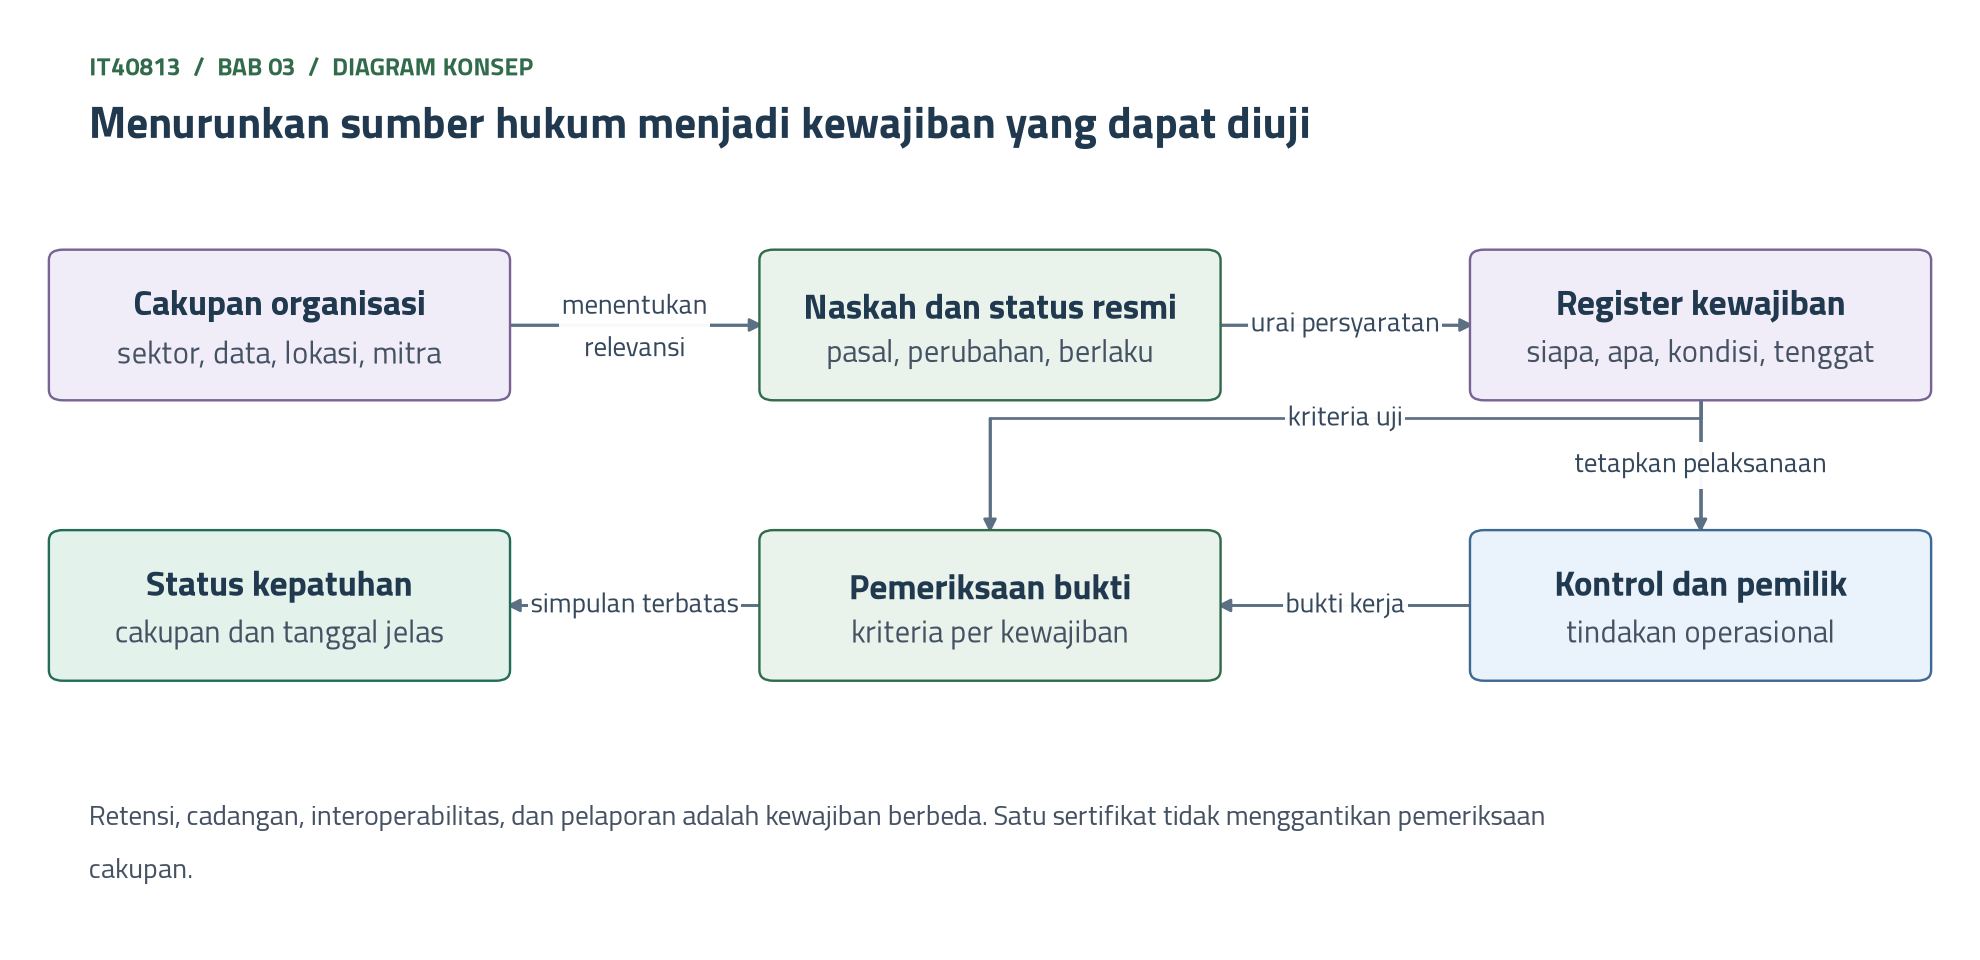
\includegraphics[width=0.96\textwidth,height=0.77\textheight,keepaspectratio]{../../figures/ch03-diagram-konsep.png}
  \label{fig:session03-ilustrasi-bab}
\end{frame}

\section{Membaca Regulasi}

\begin{frame}{\hfill}
  \centering
  \Huge{\textbf{Membaca Regulasi\\Indonesia}}
\end{frame}

\begin{frame}{{\Large Mulai dari Cakupan Organisasi}}
  \vspace{2pt}
  \footnotesize
  \begin{tabularx}{\textwidth}{|>{\raggedright\arraybackslash}p{0.14\textwidth}|>{\raggedright\arraybackslash}X|>{\raggedright\arraybackslash}X|}
    \hline
    \textbf{Pertanyaan} & \textbf{Keadaan Medikara} & \textbf{Titik awal penelusuran} \\ \hline
    Sektor & Kesehatan swasta, 36 fasilitas & UU 17/2023, PP 28/2024, Permenkes 24/2022 \\ \hline
    Jenis data & Data kesehatan, sekitar 1,2 juta kunjungan per tahun & UU PDP, data pribadi spesifik \\ \hline
    Lokasi & Sistem di rumah sakit, rencana \textit{cloud}, vendor & PP 71/2019, PP 28/2024, Pasal 56 UU PDP \\ \hline
    Model bisnis & Medikara+: 28.000 janji temu per bulan & PP 71/2019, Permenkominfo 5/2020 \\ \hline
    Mitra & BPJS Kesehatan, SATUSEHAT, asuransi, instansi & Kontrak, aturan mitra, integrasi \\ \hline
  \end{tabularx}

  \vspace{6pt}
  \small Pasal 3 Permenkes 24/2022 menyebut klinik, rumah sakit, apotek, laboratorium. Register yang
  hanya mencatat rumah sakit melewatkan 31 dari 36 fasilitas, sekitar 86 persen.
\end{frame}

\begin{frame}{{\Large Hierarki: Pasal 7 dan Pasal 8 UU 12/2011}}
  \centering
  \resizebox{!}{0.76\textheight}{\begin{tikzpicture}[
  lapis/.style={draw,rounded corners,align=center,text width=3.7cm,
    minimum height=0.7cm,font=\scriptsize,fill=blue!8},
  contoh/.style={draw,rounded corners,align=center,text width=5.2cm,
    minimum height=0.7cm,font=\scriptsize,fill=green!10},
  kosong/.style={draw,rounded corners,align=center,text width=5.2cm,
    minimum height=0.7cm,font=\scriptsize,fill=gray!35},
  judulkolom/.style={align=center,font=\scriptsize\bfseries},
  panah/.style={-{Stealth[length=2mm]},thick}
]
  \node[judulkolom] at (0,0.62) {Pasal 7 ayat (1): hierarki};
  \node[judulkolom] at (4.8,0.62) {Contoh yang dibaca Medikara};
  \node[lapis] (uud) at (0,0) {Undang-Undang Dasar 1945};
  \node[lapis] (mpr) at (0,-0.95) {Ketetapan Majelis\\ Permusyawaratan Rakyat};
  \node[lapis,fill=orange!12] (uu) at (0,-1.9) {UU atau Peraturan\\ Pemerintah Pengganti UU};
  \node[lapis,fill=orange!12] (pp) at (0,-2.85) {Peraturan Pemerintah};
  \node[lapis,fill=orange!12] (perpres) at (0,-3.8) {Peraturan Presiden};
  \node[lapis] (perda) at (0,-4.75) {Peraturan Daerah provinsi\\ dan kabupaten atau kota};
  \node[kosong] (k1) at (4.8,-0.47) {Dasar penafsiran, jarang menjadi baris register};
  \node[contoh] (c1) at (4.8,-1.9) {UU 27/2022 PDP; UU ITE dan UU 1/2024;\\ UU 17/2023 Kesehatan};
  \node[contoh] (c2) at (4.8,-2.85) {PP 71/2019 PSTE; PP 28/2024};
  \node[contoh] (c3) at (4.8,-3.8) {Perpres 82/2022 IIV; Perpres 95/2018 SPBE};
  \node[kosong] (c4) at (4.8,-4.75) {Diperiksa per lokasi fasilitas};
  \node[draw,rounded corners,align=center,text width=9.6cm,minimum height=1.1cm,font=\scriptsize,
    fill=praditagreen!15] (p8) at (2.3,-6.2) {\textbf{Pasal 8: peraturan lain yang diakui dan mengikat},
    sepanjang diperintahkan peraturan lebih tinggi atau dibentuk berdasarkan kewenangan\\
    Permenkes 24/2022; Permenkominfo 5/2020; Peraturan BSSN 1/2024; POJK 4/POJK.05/2021};
  \draw[panah] (uu) -- (c1);
  \draw[panah] (pp) -- (c2);
  \draw[panah] (perpres) -- (c3);
  \coordinate (tulang) at ($(uu.west)+(-0.3,0)$);
  \draw[thick,dashed] (uu.west) -- (tulang);
  \draw[thick,dashed] (pp.west) -- (tulang |- pp.west);
  \draw[thick,dashed] (perpres.west) -- (tulang |- perpres.west);
  \draw[panah,dashed] (tulang) -- (tulang |- p8.north);
\end{tikzpicture}
}
\end{frame}

\begin{frame}{{\Large Status di JDIH: Dua Contoh}}
  \vspace{4pt}
  \small
  \begin{itemize}
    \item Periksa nomor, tanggal berlaku, perubahan, pencabutan, dan putusan. Belum ditemukan berbeda
          dari tidak berlaku.
    \item Permenkes 24/2022 merujuk UU 29/2004, yang dicabut UU 17/2023.
    \item Pasal 453 UU 17/2023 menjaga peraturan pelaksana lama sepanjang tidak bertentangan. JDIH BPK
          mencatat status berlaku (31 Oktober 2026).
    \item PP 33/2026: BPOM menyebut diundangkan 16 Juli 2026. Basis data nonresmi menyebut mulai
          berlaku 16 Januari 2027, sisa 77 hari.
    \item Naskah resmi belum diperoleh, jadi dicatat sebagai pemantauan, bukan tenggat.
  \end{itemize}
\end{frame}

\section{PDP dan Sistem Elektronik}

\begin{frame}{\hfill}
  \centering
  \Huge{\textbf{Pelindungan Data Pribadi\\dan Sistem Elektronik}}
\end{frame}

\begin{frame}{{\Large UU PDP: Peta Pasal, Rincian di Bab 7}}
  \vspace{2pt}
  \footnotesize
  \begin{tabularx}{\textwidth}{|>{\raggedright\arraybackslash}p{0.13\textwidth}|>{\raggedright\arraybackslash}X|>{\raggedright\arraybackslash}p{0.17\textwidth}|>{\raggedright\arraybackslash}p{0.14\textwidth}|}
    \hline
    \textbf{Pasal} & \textbf{Isi ringkas} & \textbf{Register} & \textbf{Rincian} \\ \hline
    Pasal 4 & Data kesehatan termasuk data spesifik & Kolom cakupan & Bab 7 \\ \hline
    Pasal 20 & Dasar pemrosesan & K-16 & Bab 7 \\ \hline
    Pasal 39 & Mencegah akses tidak sah & K-01 & Bab 6, Bab 7 \\ \hline
    Pasal 46 & Pemberitahuan tertulis $3 \times 24$ jam & K-04 & Bab 7 \\ \hline
    Pasal 56 & Transfer ke luar wilayah hukum & K-13 & Bab 7 \\ \hline
    Pasal 57 & Sanksi administratif & Kolom akibat & Bab ini \\ \hline
    Pasal 74 & Masa penyesuaian 2 tahun & Catatan status & Bab ini \\ \hline
  \end{tabularx}

  \vspace{6pt}
  \small Putusan MK 151/PUU-XXII/2024 mengubah makna Pasal 53 ayat (1) huruf b. Status mencakup putusan.
\end{frame}

\begin{frame}{{\Large PP 71/2019 dan Permenkominfo 5/2020}}
  \vspace{4pt}
  \small
  \begin{itemize}
    \item PP 71/2019 Pasal 2 membedakan PSE lingkup publik dan privat.
    \item Pasal 6: pendaftaran sebelum sistem mulai digunakan.
    \item Pasal 24 ayat (3): gangguan serius akibat pihak lain dilaporkan dalam kesempatan pertama.
    \item Permenkominfo 5/2020 Pasal 7 ayat (2): pemutusan akses bagi PSE yang tidak mendaftar.
    \item Penafsiran bab ini: Medikara+ termasuk lingkup privat.
  \end{itemize}
\end{frame}

\begin{frame}{{\Large Analogi dan Contoh Berangka}}
  \vspace{4pt}
  \small
  \begin{itemize}
    \item Analogi: kerusakan kendaraan perlu laporan ke pemilik, asuransi, dan petugas jalan.
    \item Varian uji kontrak: misalkan kontrak vendor 12 jam, vendor melapor setelah 30 jam. Terlewati
          18 jam, sisa 42 dari 72 jam Pasal 46.
    \item 28.000 janji temu per bulan berarti 336.000 per tahun. Lokasi server utama belum menjelaskan
          seluruh pemrosesan.
    \item Pasal 57: denda paling tinggi 2 persen. Misalkan variabel Rp500 miliar, batas atas Rp10 miliar.
    \item Pasal 74: masa penyesuaian berakhir 17 Oktober 2024, sebelum insiden vendor 2025.
  \end{itemize}
\end{frame}

\begin{frame}{{\Large Kasus Medikara: Siapa PSE Medikara+?}}
  \vspace{4pt}
  \small
  \begin{itemize}
    \item Misalkan tanda daftar PSE atas nama vendor, lalu pimpinan menganggap seluruh kewajiban pindah.
    \item Kesimpulan itu mencampur dua pertanyaan: siapa mendaftar, dan siapa pengendali data.
    \item PP 28/2024 Pasal 962: penyelenggara Sistem Informasi Kesehatan merupakan pengendali data pribadi.
    \item UU PDP Pasal 37: pengendali mengawasi pihak yang terlibat dalam pemrosesan.
    \item Tim mencatat K-10 dan K-16, lalu meminta tinjauan fungsi hukum.
  \end{itemize}
\end{frame}

\section{Sektor Kesehatan}

\begin{frame}{\hfill}
  \centering
  \Huge{\textbf{Regulasi Sektor\\Kesehatan}}
\end{frame}

\begin{frame}{{\Large Rantai Tiga Tingkat}}
  \vspace{2pt}
  \footnotesize
  \begin{tabularx}{\textwidth}{|>{\raggedright\arraybackslash}p{0.22\textwidth}|>{\raggedright\arraybackslash}p{0.11\textwidth}|>{\raggedright\arraybackslash}X|}
    \hline
    \textbf{Aturan} & \textbf{Pasal} & \textbf{Isi ringkas} \\ \hline
    UU 17/2023 & 296, 297 & Tanggung jawab fasilitas; kerahasiaan; akses pasien \\ \hline
    PP 28/2024 & 779, 781 & Wajib elektronik; integrasi dengan sistem nasional \\ \hline
    PP 28/2024 & 966, 972 & Pusat data di Indonesia; transfer dengan izin Menteri \\ \hline
    Permenkes 24/2022 & 20, 21 & Keamanan, cadangan; terhubung platform kementerian \\ \hline
    Permenkes 24/2022 & 22 & Kerja sama dengan PSE berfasilitas dalam negeri \\ \hline
    Permenkes 24/2022 & 39, 42 & Simpan paling singkat 25 tahun; sanksi administratif \\ \hline
  \end{tabularx}

  \vspace{6pt}
  \small Pasal 45 Permenkes 24/2022: batas penyelenggaraan 31 Desember 2023 sudah lewat.
\end{frame}

\begin{frame}{{\Large Empat Kewajiban yang Sering Tertukar}}
  \vspace{4pt}
  \small
  \begin{itemize}
    \item Retensi: berapa lama data dipertahankan.
    \item Cadangan: bagaimana data dipulihkan saat salinan utama rusak.
    \item Interoperabilitas: apakah data sampai dan terbaca di sistem tujuan.
    \item Pelaporan: siapa perlu diberi tahu ketika ada kejadian.
    \item Analogi: salinan di lemari kedua membantu saat lemari pertama rusak, tetapi tidak menjamin
          arsip tetap terbaca sampai akhir masa simpan.
  \end{itemize}
\end{frame}

\begin{frame}{{\Large Dua Contoh Berangka}}
  \vspace{4pt}
  \small
  \begin{itemize}
    \item Misalkan 5 rumah sakit memakai versi SIMRS berbeda. Satu prosedur retensi perlu bukti pada tiap
          sistem.
    \item Sekitar 1,2 juta kunjungan per tahun selama 25 tahun berarti sekitar 30 juta catatan.
    \item Kunjungan terakhir 2 Maret 2026 berarti batas simpan paling singkat 2 Maret 2051.
    \item Misalkan klinik mengirim 1.000 catatan dan 40 ditolak platform, atau 4 persen.
    \item Di 18 klinik, 720 dari 18.000 catatan perlu ditelusuri.
  \end{itemize}
\end{frame}

\begin{frame}{{\Large Bolehkah Disimpan di Luar Negeri?}}
  \centering
  \resizebox{!}{0.76\textheight}{\begin{tikzpicture}[
  tanya/.style={draw,rounded corners,align=center,text width=6.0cm,
    minimum height=1.0cm,font=\scriptsize,fill=orange!12},
  mulai/.style={draw,rounded corners,align=center,text width=6.0cm,
    minimum height=0.8cm,font=\scriptsize,fill=blue!8},
  hasil/.style={draw,rounded corners,align=center,text width=6.0cm,
    minimum height=0.8cm,font=\scriptsize,fill=green!10},
  henti/.style={draw,rounded corners,align=center,text width=3.7cm,
    minimum height=1.0cm,font=\scriptsize,fill=red!22},
  perbaiki/.style={draw,rounded corners,align=center,text width=3.7cm,
    minimum height=1.0cm,font=\scriptsize,fill=gray!35},
  label/.style={font=\scriptsize,fill=white,inner sep=1pt},
  panah/.style={-{Stealth[length=2mm]},thick}
]
  \node[mulai] (a) at (0,0) {Usulan: rekam medis atau Data Kesehatan disimpan memakai jasa pihak lain};
  \node[tanya] (b) at (0,-1.75) {Pusat data, termasuk salinan cadangan, berada di dalam wilayah
    Indonesia?\\ {\tiny\mdseries PP 28/2024 Pasal 966 ayat (2) dan (5) huruf a}};
  \node[tanya] (c) at (0,-3.7) {Perjanjian memuat kerahasiaan dan tingkat layanan, dan data tetap
    dikendalikan penuh oleh penyelenggara?\\ {\tiny\mdseries PP 28/2024 Pasal 966 ayat (5) huruf b sampai d}};
  \node[tanya] (d) at (0,-5.65) {PSE mendapat rekomendasi Kementerian Kesehatan dan menandatangani
    larangan pemanfaatan data?\\ {\tiny\mdseries Permenkes 24/2022 Pasal 22 ayat (2) sampai (4)}};
  \node[hasil] (e) at (0,-7.35) {Lanjut ke penilaian teknis, uji pemulihan, dan pengumpulan bukti};
  \node[henti] (b2) at (5.6,-1.75) {Ini transfer ke luar wilayah: tujuan spesifik, izin Menteri, syarat
    transfer data pribadi\\ {\tiny\mdseries PP 28/2024 Pasal 972; UU PDP Pasal 56}};
  \node[perbaiki] (c2) at (5.6,-3.7) {Perbaiki perjanjian sebelum persetujuan kontrak};
  \node[perbaiki] (d2) at (5.6,-5.65) {Lengkapi rekomendasi sebelum kerja sama dimulai};
  \draw[panah] (a) -- (b);
  \draw[panah] (b) -- node[label,right] {Ya} (c);
  \draw[panah] (c) -- node[label,right] {Ya} (d);
  \draw[panah] (d) -- node[label,right] {Ya} (e);
  \draw[panah] (b) -- node[label,above] {Tidak} (b2);
  \draw[panah] (c) -- node[label,above] {Tidak} (c2);
  \draw[panah] (d) -- node[label,above] {Tidak} (d2);
\end{tikzpicture}
}
\end{frame}

\begin{frame}{{\Large Kasus Medikara: Lapis Kewajiban}}
  \vspace{4pt}
  \small
  \begin{itemize}
    \item Misalkan vendor menawarkan penyimpanan luar negeri Rp420 juta per tahun, dari Rp600 juta. Hemat
          Rp180 juta, atau 30 persen.
    \item Kontrak Rp420 juta melewati batas Rp400 juta pada Bab 2, sehingga naik ke direksi.
    \item Usulan berhenti pada pertanyaan pertama: pusat data di dalam wilayah Indonesia?
    \item Harga lebih rendah bukan alasan menerima desain sebelum kewajiban sektor dinilai.
    \item Pilihan: tawar ulang fasilitas dalam negeri, atau pisahkan data bukan rekam medis setelah dinilai.
  \end{itemize}
\end{frame}

\section{Siber dan IIV}

\begin{frame}{\hfill}
  \centering
  \Huge{\textbf{Keamanan Siber Nasional\\dan Infrastruktur\\Informasi Vital}}
\end{frame}

\begin{frame}{{\Large Sektor Berbeda dari Penetapan Sistem}}
  \vspace{4pt}
  \small
  \begin{itemize}
    \item Perpres 82/2022 Pasal 4: kesehatan termasuk sektor IIV.
    \item Pasal 6: identifikasi paling sedikit 1 kali setahun, dilaporkan, diverifikasi, lalu ditetapkan.
    \item Peraturan BSSN 1/2024 Pasal 7 dan 8: penyelenggara membentuk tim tanggap insiden organisasi.
    \item Pasal 15: insiden paling sedikit berisiko tinggi dilaporkan; $1 \times 24$ jam bila terjadi pada IIV.
    \item Sistem Medikara tidak diasumsikan sudah ditetapkan sebagai IIV.
  \end{itemize}
\end{frame}

\begin{frame}{{\Large Analogi dan Dua Contoh}}
  \vspace{4pt}
  \small
  \begin{itemize}
    \item Analogi: masuk kawasan rawan banjir tidak berarti setiap bangunan berisiko sama.
    \item Misalkan pendaftaran berhenti dua jam di 1 dari 18 klinik. Tim mengklasifikasikan dampak dulu.
    \item Di bawah risiko tinggi: tidak masuk Pasal 15 ayat (3), tetapi tetap dicatat.
    \item Misalkan 5 rumah sakit dan sekitar 640 dokter bergantung pada satu layanan identitas.
    \item Ketergantungan itu masuk bahan identifikasi tahunan Pasal 6.
  \end{itemize}
\end{frame}

\begin{frame}{{\Large Satu Kejadian, Beberapa Jam}}
  \centering
  \resizebox{0.97\textwidth}{!}{\begin{tikzpicture}[
  kontrak/.style={draw,rounded corners,align=center,text width=1.85cm,
    minimum height=1.35cm,font=\scriptsize,fill=orange!12},
  hukum/.style={draw,rounded corners,align=center,text width=1.85cm,
    minimum height=1.55cm,font=\scriptsize,fill=blue!8},
  mulai/.style={draw,rounded corners,align=center,text width=1.55cm,
    minimum height=1.35cm,font=\scriptsize,fill=praditagreen!15},
  waktu/.style={align=center,font=\scriptsize\bfseries},
  jam/.style={align=center,font=\tiny},
  panah/.style={-{Stealth[length=2mm]},thick}
]
  \draw[panah] (-0.2,0) -- (11.15,0);
  \foreach \posisi in {0,2.0,4.1,6.0,8.1,10.2}
    \draw[thick] (\posisi,0.1) -- (\posisi,-0.1);
  \node[mulai] (mulai) at (0,1.15) {Kegagalan terjadi dan ditemukan};
  \node[kontrak] (a) at (2.0,1.15) {Medikara ke mitra asuransi\\ {\tiny\mdseries kontrak, misalkan}};
  \node[kontrak] (b) at (4.1,1.15) {Vendor ke Medikara\\ {\tiny\mdseries kontrak, misalkan}};
  \node[hukum] (c) at (6.0,-1.3) {Tim tanggap ke tim sektoral\\ {\tiny\mdseries Perpres 82/2022
    Pasal 13, hanya bila IIV}};
  \node[hukum] (d) at (8.1,-1.3) {Pengendali ke subjek data dan lembaga\\ {\tiny\mdseries UU PDP
    Pasal 46}};
  \node[hukum] (e) at (10.2,-1.3) {Mitra asuransi ke OJK\\ {\tiny\mdseries POJK Pasal 31, kejadian
    pada TI mitra}};
  \draw (mulai) -- (0,0.1);
  \draw (a) -- (2.0,0.1);
  \draw (b) -- (4.1,0.1);
  \draw (c) -- (6.0,-0.1);
  \draw (d) -- (8.1,-0.1);
  \draw (e) -- (10.2,-0.1);
  \node[jam] at (0,-0.42) {Jumat 20.00};
  \node[waktu] at (2.0,-0.28) {1 jam};
  \node[jam] at (2.0,-0.55) {Jumat 21.00};
  \node[waktu] at (4.1,-0.28) {12 jam};
  \node[jam] at (4.1,-0.55) {Sabtu 08.00};
  \node[waktu] at (6.0,0.4) {$1 \times 24$ jam};
  \node[jam] at (6.0,0.68) {Sabtu 20.00};
  \node[waktu] at (8.1,0.4) {$3 \times 24$ jam};
  \node[jam] at (8.1,0.68) {Senin 20.00};
  \node[waktu] at (10.2,0.4) {5 hari kerja};
  \node[jam] at (10.2,0.68) {Jumat berikutnya};
\end{tikzpicture}
}

  \vspace{8pt}
  \raggedright\small Asumsi sama dengan Bab 7: kejadian dan penemuan bersamaan. Skala tidak proporsional.
  Angka kontrak adalah pengandaian.
\end{frame}

\begin{frame}{{\Large Kasus Medikara: Insiden dan Jam Lapor}}
  \vspace{4pt}
  \small
  \begin{itemize}
    \item Varian uji kontrak: vendor menemukan akun dipakai di luar penugasan Jumat 20.00, memberi tahu Minggu 02.00.
    \item Kontrak 12 jam terlewati 18 jam. Batas Pasal 46 Senin 20.00, tersisa 42 jam.
    \item Koordinator membuka K-04, K-05, dan K-09. Satu laporan tidak dipakai untuk semua penerima.
    \item Data latihan Bab 1: 8 malam, baru diketahui hari ke-11. Rentang 72 jam setara 3 hari.
    \item Tim mencatat waktu kejadian dan waktu diketahui; fungsi hukum menetapkan batas konservatif. PP 33/2026 Pasal 114 ayat (2) hanya dipantau dari salinan pihak ketiga.
  \end{itemize}
\end{frame}

\section{Mitra: OJK dan SPBE}

\begin{frame}{\hfill}
  \centering
  \Huge{\textbf{Regulasi yang Mengikat\\Mitra: OJK dan SPBE}}
\end{frame}

\begin{frame}{{\Large Aturan Mitra Tidak Otomatis Berlaku}}
  \vspace{4pt}
  \small
  \begin{itemize}
    \item POJK 4/POJK.05/2021 Pasal 2: perusahaan asuransi termasuk Lembaga Jasa Keuangan Nonbank
          (LJKNB).
    \item Pasal 21: LJKNB tetap bertanggung jawab dan mengawasi penyedia jasa TI.
    \item Pasal 31: kejadian kritis dilaporkan paling lambat 5 hari kerja setelah diketahui.
    \item Perpres 95/2018 Pasal 70: evaluasi SPBE ditujukan bagi instansi pusat dan pemerintah daerah.
    \item Menerima klaim tidak mengubah rumah sakit menjadi lembaga jasa keuangan.
  \end{itemize}
\end{frame}

\begin{frame}{{\Large Mengikat Langsung atau Lewat Kontrak}}
  \centering
  \resizebox{0.95\textwidth}{!}{\begin{tikzpicture}[
  aturan/.style={draw,rounded corners,align=center,text width=2.2cm,
    minimum height=1.05cm,font=\scriptsize,fill=blue!8},
  mitra/.style={draw,rounded corners,align=center,text width=2.2cm,
    minimum height=1.05cm,font=\scriptsize,fill=orange!12},
  pusat/.style={draw,rounded corners,align=center,text width=2.0cm,
    minimum height=1.2cm,font=\scriptsize\bfseries,fill=praditagreen!15},
  akhir/.style={draw,rounded corners,align=center,text width=1.8cm,
    minimum height=1.05cm,font=\scriptsize,fill=green!10},
  label/.style={font=\tiny,inner sep=1pt},
  panah/.style={-{Stealth[length=2mm]},thick}
]
  \node[aturan,text width=5.6cm] (langsung) at (1.65,2.0) {Aturan yang mencakup Medikara sendiri:
    UU PDP, UU 17/2023, PP 28/2024, Permenkes 24/2022, PP 71/2019};
  \node[aturan] (ojk) at (-0.2,0) {POJK 4/POJK.05/2021};
  \node[mitra] (asuransi) at (3.3,0) {Perusahaan asuransi mitra (LJKNB)};
  \node[pusat] (medikara) at (6.7,0) {Medikara};
  \node[akhir] (vendor) at (9.9,0) {Vendor Medikara+ dan penyedia \textit{cloud}};
  \node[aturan] (spbe) at (-0.2,-2.0) {Perpres 95/2018 tentang SPBE};
  \node[mitra] (instansi) at (3.3,-2.0) {Instansi pemerintah mitra};
  \draw[panah] (ojk) -- node[label,above=1pt] {mengikat} (asuransi);
  \draw[panah] (spbe) -- node[label,above=1pt] {mengikat} (instansi);
  \draw[panah,dashed] (asuransi) -- node[label,above=1pt] {kontrak} (medikara);
  \draw[panah,dashed] (instansi) -| node[label,pos=0.25,above=1pt] {perjanjian} (medikara);
  \draw[panah,dashed] (medikara) -- node[label,above=1pt] {kontrak} (vendor);
  \draw[panah] (langsung.east) -| node[label,pos=0.25,above=1pt] {mengikat langsung} (medikara.north);
  \draw (6.0,-2.75) -- (6.7,-2.75) node[right,font=\tiny] {garis penuh: aturan berlaku langsung};
  \draw[dashed] (6.0,-3.05) -- (6.7,-3.05) node[right,font=\tiny] {garis putus: syarat mengalir lewat kontrak};
\end{tikzpicture}
}
\end{frame}

\begin{frame}{{\Large Analogi dan Dua Contoh}}
  \vspace{4pt}
  \small
  \begin{itemize}
    \item Analogi: pemasok makanan ke sekolah tidak menjadi sekolah, tetapi kontraknya dapat lebih ketat.
    \item Misalkan mitra asuransi meminta laporan gangguan dalam satu jam.
    \item Misalkan dari 12 gangguan terakhir hanya 2 tepat waktu, sekitar 17 persen. Statusnya tidak memenuhi.
    \item Pilihannya: perbaiki deteksi atau tawar ulang klausul.
    \item Misalkan rumah sakit pemerintah meminta format bukti tertentu. Tim menelusuri dasarnya dulu.
  \end{itemize}
\end{frame}

\begin{frame}{{\Large Akibat Pelanggaran Menurut Sumber}}
  \vspace{2pt}
  \footnotesize
  \begin{tabularx}{\textwidth}{|>{\raggedright\arraybackslash}p{0.29\textwidth}|>{\raggedright\arraybackslash}X|}
    \hline
    \textbf{Sumber} & \textbf{Akibat} \\ \hline
    UU PDP Pasal 57 & Peringatan, penghentian sementara, penghapusan data, denda paling tinggi 2 persen \\ \hline
    PP 71/2019 Pasal 100 & Teguran, denda, penghentian sementara, pemutusan akses, dikeluarkan dari daftar \\ \hline
    Permenkes 24/2022 Pasal 42 & Teguran, rekomendasi pencabutan atau pencabutan status akreditasi \\ \hline
    Kontrak mitra (misalkan) & Denda layanan, kewajiban perbaikan, penghentian kerja sama \\ \hline
    Standar sukarela (misalkan) & Temuan audit, pembekuan atau pencabutan sertifikat \\ \hline
  \end{tabularx}

  \vspace{6pt}
  \small Kewajiban hukum tidak dapat dihapus lewat kesepakatan vendor. Standar yang disebut dalam perjanjian
  menjadi kewajiban kontrak.
\end{frame}

\section{Register Kewajiban}

\begin{frame}{\hfill}
  \centering
  \Huge{\textbf{Register Kewajiban\\Kepatuhan}}
\end{frame}

\begin{frame}{{\Large Register: Siapa, Apa, Kapan, Bukti}}
  \vspace{4pt}
  \small
  \begin{itemize}
    \item Satu pasal dapat menjadi beberapa baris. Satu kontrol dapat mendukung beberapa kewajiban.
    \item ISO 37301:2021 memberi kerangka sistem manajemen kepatuhan. Register adalah salah satu alatnya.
    \item Analogi: daftar pindah kantor berguna bila tiap tugas punya pemilik, tenggat, dan tanda terima.
    \item Register contoh, 16 baris: 2 terverifikasi memenuhi, 4 memenuhi sebagian, 2 tidak memenuhi,
          7 belum diverifikasi, 1 tidak berlaku.
    \item Sebanyak 7 baris, atau sekitar 44 persen, belum berbukti. Sisanya tidak otomatis patuh.
  \end{itemize}
\end{frame}

\begin{frame}{{\Large Jejak Satu Baris Register}}
  \centering
  \vspace{6pt}
  \resizebox{0.97\textwidth}{!}{\begin{tikzpicture}[
  kotak/.style={draw,rounded corners,align=center,text width=1.95cm,
    minimum height=1.45cm,font=\scriptsize,fill=blue!8},
  label/.style={font=\tiny,fill=white,inner sep=1pt},
  panah/.style={-{Stealth[length=2mm]},thick}
]
  \node[kotak,fill=praditagreen!15] (a) at (0,0) {\textbf{Sumber}\\ UU PDP Pasal 39: cegah akses tidak sah};
  \node[kotak,fill=orange!12] (b) at (2.4,0) {\textbf{K-01}\\ Kewajiban dengan pemilik Medikara+};
  \node[kotak] (c) at (4.8,0) {\textbf{AC-01}\\ Peninjauan hak akses bulanan};
  \node[kotak] (d) at (7.2,0) {\textbf{B-01}\\ 6 dari 30 akun sampel belum dicabut};
  \node[kotak,fill=green!10] (e) at (9.6,0) {\textbf{Status}\\ Memenuhi sebagian, cakupan dan tanggal jelas};
  \node[kotak,fill=red!22,minimum height=0.95cm] (r) at (4.8,-2.05) {\textbf{R-01}\\ Akses vendor berlebihan};
  \draw[panah] (a) -- (b);
  \draw[panah] (b) -- (c);
  \draw[panah] (c) -- (d);
  \draw[panah] (d) -- (e);
  \draw[panah] (c) -- node[label,right] {menurunkan} (r);
  \draw[panah,dashed] (b.south) |- (r.west);
  \draw[panah,dashed] (e.south) -- (9.6,-3.0) -- node[label,below] {aturan, kegiatan, atau vendor berubah: baris ditinjau ulang} (0,-3.0) -- (a.south);
\end{tikzpicture}
}

  \vspace{10pt}
  \raggedright\small Bab 1: 6 dari 30 akun sampel belum dicabut; peninjauan berikutnya mencabut 24 dari 120 akun.
\end{frame}

\begin{frame}{{\Large Satu Pasal, Tiga Hal yang Diuji}}
  \vspace{2pt}
  \footnotesize
  \begin{tabularx}{\textwidth}{|>{\raggedright\arraybackslash}p{0.2\textwidth}|>{\raggedright\arraybackslash}X|>{\raggedright\arraybackslash}X|}
    \hline
    \textbf{Unsur pasal} & \textbf{Tindakan yang diuji} & \textbf{Bukti} \\ \hline
    Tempat berbeda & Cadangan di luar lokasi tiap fasilitas & Inventaris lokasi cadangan \\ \hline
    Periodik & Cadangan berjalan sesuai jadwal & Catatan cadangan dan uji pemulihan \\ \hline
    Prosedur tertulis & Prosedur ditetapkan tiap fasilitas & Prosedur operasional yang disahkan \\ \hline
  \end{tabularx}

  \vspace{8pt}
  \small
  \begin{itemize}
    \item Sumber: Pasal 20 ayat (4) dan (5) Permenkes 24/2022.
    \item Misalkan satu uji pemulihan per fasilitas per triwulan: 36 fasilitas, 144 uji setahun.
    \item Angka itu menjadi dasar menilai beban kerja 52 staf TI.
  \end{itemize}
\end{frame}

\begin{frame}{{\Large Contoh Register dan Batas Sertifikat}}
  \vspace{2pt}
  \scriptsize
  \begin{tabularx}{\textwidth}{|>{\raggedright\arraybackslash}p{0.26\textwidth}|>{\raggedright\arraybackslash}X|>{\raggedright\arraybackslash}X|}
    \hline
    \textbf{ID dan dasar} & \textbf{Pemilik dan tindakan} & \textbf{Bukti serta status} \\ \hline
    K-01, UU PDP Pasal 39 & Pemilik Medikara+ mencegah akses tidak sah & Hasil AC-01; memenuhi sebagian \\ \hline
    K-02, Permenkes Pasal 20 & TI dan rekam medis menguji cadangan & Laporan uji; belum diverifikasi \\ \hline
    K-03, Permenkes Pasal 39 & Rekam medis menjaga retensi & Jadwal retensi; memenuhi sebagian \\ \hline
    K-04, UU PDP Pasal 46 & Pengendali menyiapkan pemberitahuan & Kronologi, salinan; belum diverifikasi \\ \hline
    K-05, kontrak vendor & Pengelola vendor menagih laporan 12 jam & Rekam komunikasi; tidak memenuhi \\ \hline
    K-15, POJK Pasal 31 & Analis regulasi mencatat alasan & Pasal 2 POJK; tidak berlaku \\ \hline
  \end{tabularx}

  \vspace{6pt}
  \small ISO/IEC 27001 menilai sistem manajemen dalam ruang lingkup tertentu. Satu sertifikat tidak menggantikan
  pemeriksaan cakupan.
\end{frame}

\section{Aktivitas dan Penutup}

\begin{frame}{{\Large Aktivitas: Register Kewajiban}}
  \vspace{4pt}
  \small
  \textbf{Tujuan:} daftar kewajiban yang jelas cakupan, pemilik, dan buktinya.

  \vspace{4pt}
  \begin{itemize}
    \item Analis regulasi memimpin pembacaan pasal.
    \item Pemilik konteks menetapkan fungsi pemilik.
    \item Analis teknologi menilai implikasi sistem.
    \item Analis risiko menuliskan konsekuensi dan keterkaitan skenario.
    \item Register minimal: UU PDP, rekam medis elektronik, PSTE, SATUSEHAT, pelaporan insiden siber.
  \end{itemize}
\end{frame}

\begin{frame}{{\Large Aktivitas: Langkah dan Penilaian}}
  \vspace{4pt}
  \small
  \begin{itemize}
    \item Tentukan cakupan, lalu periksa sumber resmi dan status tiap aturan.
    \item Pilih sedikitnya 10 kewajiban. Isi pemilik, kondisi, tenggat, bukti, status, dan ID kontrol.
    \item Tinjau silang satu baris: pemeriksa menyimpulkan status tanpa menebak maksud penulis.
    \item Luaran masuk C1, dipakai ulang pada Bab 5, Bab 7, dan Bab 12. Berkas: \texttt{sources/chapter03/}.
    \item Nilai: cakupan dan sumber 30 persen, dapat diuji 30 persen, pemilik dan bukti 25 persen,
          konsistensi status 15 persen.
  \end{itemize}
\end{frame}

\begin{frame}{{\Large Ringkasan}}
  \vspace{4pt}
  \small
  \begin{itemize}
    \item Kepatuhan dimulai dari cakupan, bukan dari daftar sertifikat: 36 fasilitas, bukan 5 rumah sakit.
    \item Naskah resmi, status, putusan, dan ketentuan penutup dibaca bersama.
    \item Retensi, cadangan, interoperabilitas, dan pelaporan adalah kewajiban berbeda. Batas $3 \times 24$ jam
          tidak sama dengan $1 \times 24$ jam.
    \item Hukum membawa sanksi, kontrak membawa akibat perjanjian, standar mengikat karena dipilih.
    \item Kewajiban baru dapat diperiksa setelah organisasi menjelaskan pekerjaan dan cara membuktikannya.
  \end{itemize}
\end{frame}

\begin{frame}{{\Large Latihan dan Bacaan}}
  \vspace{2pt}
  \footnotesize
  \begin{enumerate}
    \item Sebuah klinik mitra menyimpan rekam medis di layanan \textit{cloud} luar negeri. Kewajiban apa saja
          yang perlu diperiksa, dan pada peraturan mana?
    \item Tulis ulang satu pasal UU PDP menjadi kewajiban yang dapat diperiksa auditor: siapa melakukan apa,
          kapan, dan apa buktinya.
    \item Jelaskan mengapa sertifikat ISO/IEC 27001 tidak otomatis membuktikan kepatuhan pada UU PDP.
  \end{enumerate}

  \vspace{6pt}
  \textbf{Bacaan:} \href{https://peraturan.bpk.go.id/Details/229798/uu-no-27-tahun-2022}{UU PDP};
  \href{https://peraturan.bpk.go.id/Details/294077}{PP 28/2024};
  \href{https://peraturan.go.id/files/bn829-2022.pdf}{Permenkes 24/2022};
  \href{https://peraturan.go.id/files/ps82-2022.pdf}{Perpres 82/2022};
  \href{https://peraturan.go.id/files/peraturan-bssn-no-1-tahun-2024.pdf}{BSSN 1/2024}.
\end{frame}

\end{document}
